\documentclass[]{article}
\usepackage[utf8]{inputenc}
\usepackage[spanish]{babel}
\usepackage{graphicx}
\usepackage{hyperref}
\usepackage{xcolor}
\usepackage{listings}
\graphicspath{{./imagenes/}}

\colorlet{punct}{red!60!black}
\definecolor{background}{HTML}{EEEEEE}
\definecolor{delim}{RGB}{20,105,176}
\colorlet{numb}{magenta!60!black}
\definecolor{codegreen}{rgb}{0,0.6,0}
\definecolor{codegray}{rgb}{0.5,0.5,0.5}
\definecolor{codepurple}{rgb}{0.58,0,0.82}
\definecolor{backcolour}{rgb}{0.95,0.95,0.92}

\lstset{
	frame = shadowbox, 
	basicstyle=\small,
	inputencoding=utf8,
	extendedchars=true,
	breaklines, 
	numbers = left, 
	literate={ó}{{\'o}}1 {á}{{\'a}}1 {é}{{\'e}}1 {í}{{\'i}}1 {ú}{{\'u}}1 {ñ}{{\~n}}1,
	commentstyle=\color{codegreen},
	keywordstyle=\color{magenta},
	numberstyle=\tiny\color{codegray},
	stringstyle=\color{codepurple},
}


\lstdefinelanguage{C}{
	backgroundcolor=\color{backgroundColour},   
	commentstyle=\color{mGreen},
	morecomment=[l]{//}, %use comment-line-style!
	morecomment=[s]{/*}{*/}, %for multiline comments
	keywordstyle=\color{magenta},
	numberstyle=\tiny\color{mGray},
	stringstyle=\color{mPurple},
	basicstyle=\footnotesize,
	breakatwhitespace=false,         
	breaklines=true,                 
	captionpos=b,                    
	keepspaces=true,                 
	numbers=left,                    
	numbersep=5pt,                  
	showspaces=false,                
	showstringspaces=false,
	showtabs=false,                  
	tabsize=2,
}

\lstdefinelanguage{json}{
	basicstyle=\normalfont\ttfamily,
	numbers=left,
	numberstyle=\scriptsize,
	stepnumber=1,
	numbersep=8pt,
	showstringspaces=false,
	breaklines=true,
	frame=lines,
	backgroundcolor=\color{background},
	literate=
	*{0}{{{\color{numb}0}}}{1}
	{1}{{{\color{numb}1}}}{1}
	{2}{{{\color{numb}2}}}{1}
	{3}{{{\color{numb}3}}}{1}
	{4}{{{\color{numb}4}}}{1}
	{5}{{{\color{numb}5}}}{1}
	{6}{{{\color{numb}6}}}{1}
	{7}{{{\color{numb}7}}}{1}
	{8}{{{\color{numb}8}}}{1}
	{9}{{{\color{numb}9}}}{1}
	{:}{{{\color{punct}{:}}}}{1}
	{,}{{{\color{punct}{,}}}}{1}
	{\{}{{{\color{delim}{\{}}}}{1}
	{\}}{{{\color{delim}{\}}}}}{1}
	{[}{{{\color{delim}{[}}}}{1}
	{]}{{{\color{delim}{]}}}}{1},
}

\begin{document}
	\begin{titlepage}
	\centering
	
\includegraphics[width=0.15\textwidth]{ITCH}\par\vspace{1cm}
	{\textsc{INSTITUTO TECNOLÓGICO DE CHIHUAHUA CAMPUS I} \par}
	\vspace{0.5cm}
	{\textsc{Laboratorio de Innovación Intel} \par}
	\vspace{1cm}
	\vspace{1.5cm}
	{\huge\bfseries MANUAL DE USUARIO AZURE SPHERE MT3620 \par}
	\vspace{2cm}
	{\Large Javier Pérez Macias\par}
	\vfill
	% Bottom of the page
	{\large \today\par}
\end{titlepage}
	\pagebreak
	\tableofcontents
	\section{Introducción}

La Azure Sphere MT3620 development kit es uno de los primeros microcontroladores certificados para utilizar la plataforma Azure Sphere, esta es desarrollada por Microsoft, consiste en una plataforma de aplicación de alto nivel para la comunicación de dispositivos conectados a internet, todo con un enfoque en la seguridad.
\subsection{Azure Sphere}
La plataforma incluye una conexión entre un microcontrolador, un sistema operativo Linux modificado y seguridad continua basada en la nube. La principal apuesta de esta plataforma es la seguridad de alto nivel que proveen. Está diseñada con base en siete propiedades:
\begin{itemize}
	\item 
	\textbf{Actualizaciones de seguridad:}estos dispositivos se actualizan automáticamente para corregir vulnerabilidades detectadas, esto no requiere intervención del usuario o fabricante.
	\item 
	\textbf{Reporte de errores:} Los dispositivos reportan fallos automáticamente a un sistema en la nube.
	\item
	\textbf{Autenticación sin contraseña:} La plataforma usa certificados firmados; estos se validan por medio de una llave criptográfica, lo que provee una mayor seguridad que el usar contraseñas.
	\item
	\textbf{Niveles de seguridad:} La defensa de esta plataforma es tener varias capas de seguridad, una encima de otra, perfectas para mitigar daños.
	\item
	\textbf{Hardware Seguro:} Cada microcontrolador tiene su identificador único con su propia llave criptográfica, por lo que se usa como un recurso en el que siempre puedes confiar para el sistema de criptografía, lo que normalmente se le llama Root of Trust (RoT).
	\item
	\textbf{Compartimentos dinámicos:}  Limita el alcance de cualquier error. Los microcontroladores de esta plataforma contienen muros físicos que prevén a un error propagarse a otros componentes.
	\item
	\textbf{Pocos componentes críticos a la seguridad:} La mayoría del software se mantiene fuera de la base de computador confiable, solo pocos sistemas que provee Microsoft entran a la seguridad del sistema.
\end{itemize}
\begin{figure}[h]
	\centering
	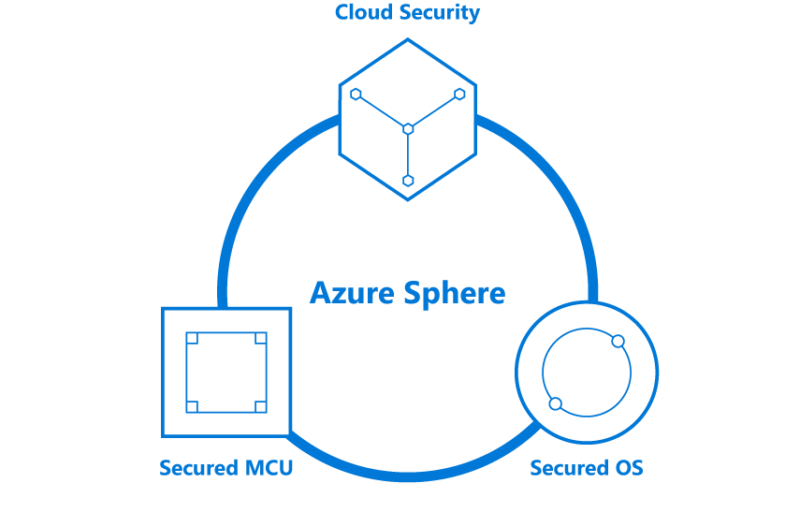
\includegraphics[scale=1.5]{azuresphere}
	\caption{Descripción grafica de la plataforma}
\end{figure}
	\section{Arquitectura}
\begin{itemize}
	\item
	ARM Cortex A7 core @500MHz, 4MB RAM
	\item
	2 ARM Cortex M4 core @200MHz, 64KB RAM
	\item
	4 Interfaces ISU, pueden ser configuradas como I2C hasta 1MHz, SPI hasta 40MHz, UART hasta 3Mbps
	\item
	RTC con recipiente de batería CR2032
	\item
	4 Entradas y salidas ADC de 12 bits
	\item
	Un puerto I2S, maestro o esclavo, también soporta TDM esclavo
	\item
	Puerto micro-USB de alimentación, 5V/1A
	\item
	Conectividad Wi-Fi 2.4/5GHz banda dual 802.11 b/g/n
	\item
	Jack DC de 5V/1A
	\item
	Temperatura de operación -40~85°C
\end{itemize}	
\begin{figure}[h]
	\centering
	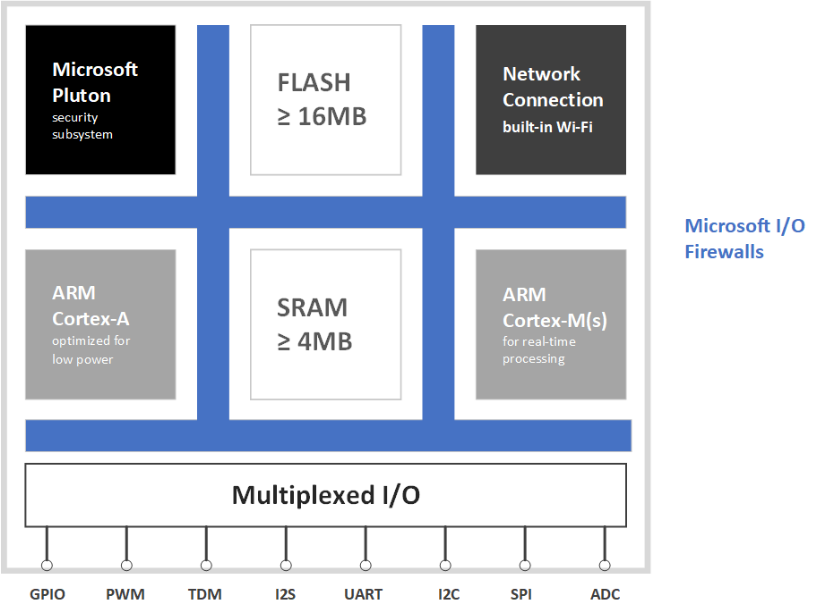
\includegraphics[scale=1.25]{arquitectura}
	\caption{Arquitectura del hardware}
\end{figure}

\begin{figure}[h]
	\centering
	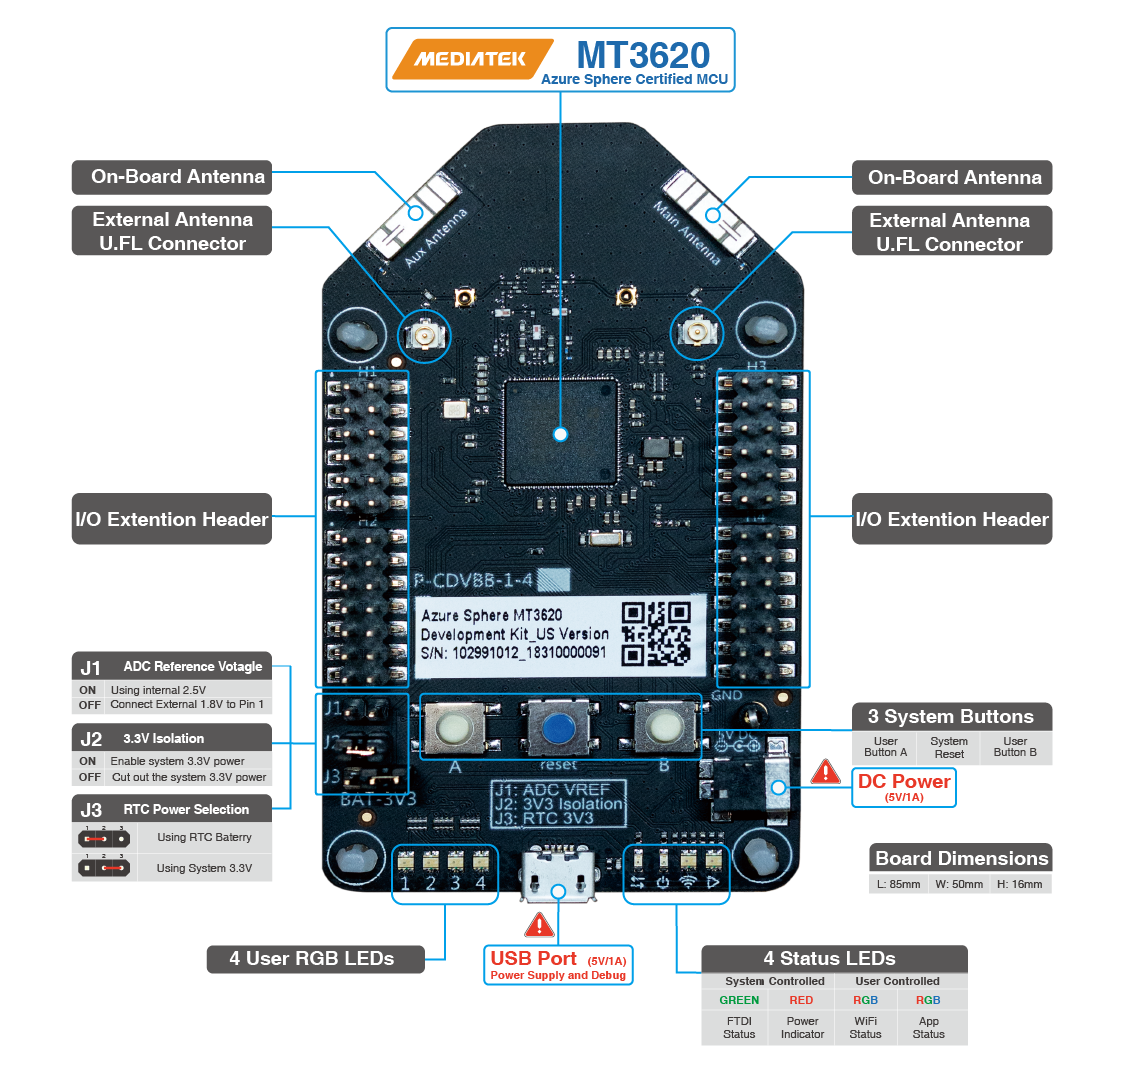
\includegraphics[scale=.50]{diagrama}
	\caption{Diagrama de la Azure Sphere MT3620 Development Kit}
\end{figure}

\begin{figure}[h]
	\centering
	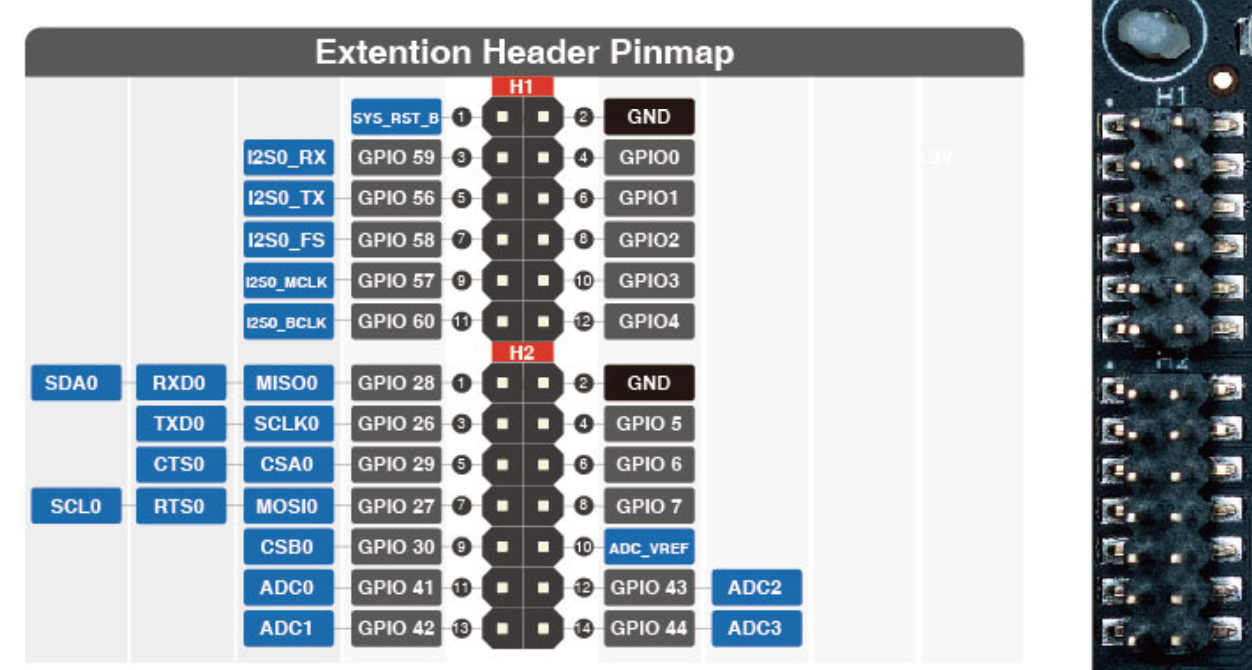
\includegraphics[scale=.30]{pins1}
	\caption{Mapa de pines H1-H2}
\end{figure}

\begin{figure}[h]
	\centering
	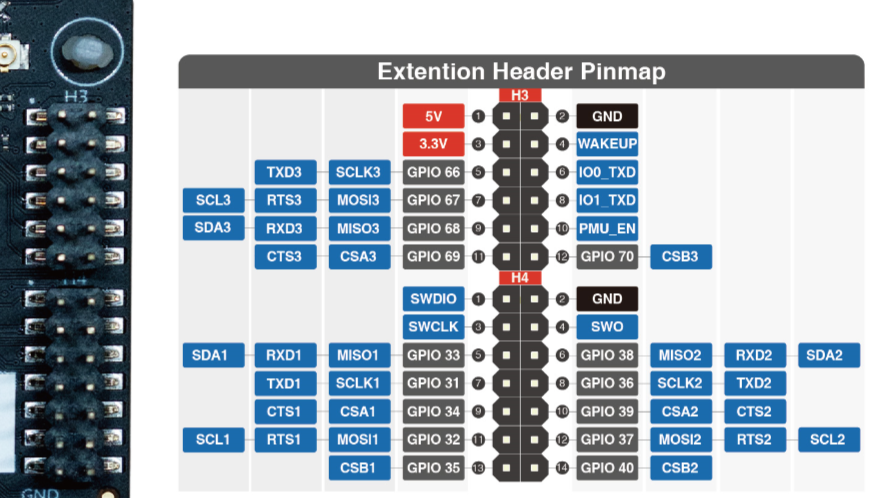
\includegraphics[scale=.50]{pins2}
	\caption{Mapa de pines H3-H4}
\end{figure}
	\section{Herramientas a instalar}

\begin{itemize}
	\item 
	Puerto USB
	\item
	Sistema Operativo: Windows 10/11 o 
	distribucion \href{https://releases.ubuntu.com/jammy/}{Ubuntu 22.04} 
	\item 
	Lenguaje de programación: C
	\item 
	Entorno de Desarrollo: \href{https://visualstudio.microsoft.com/es/}{Visual Studio}, 
	\href{https://code.visualstudio.com/}{Visual Studio Code} o Terminal
	\item
	Azure Sphere SDK en \href{https://learn.microsoft.com/en-us/azure-sphere/install/install-sdk}{Windows} o \href{https://learn.microsoft.com/en-us/azure-sphere/install/install-sdk-linux}{Linux}
\end{itemize}

\subsection{Instalación}
\subsubsection{Windows}
\subsubsection*{Visual Studio}
\begin{enumerate}
	\item 
	Conectar el microcontrolador, Windows automaticamente instalara los drivers necesarios (En caso de que no se puede usar los drivers de \href{https://www.ftdichip.com/Drivers/VCP.htm}{FTDI})
	\item 
	Instalar el \href{https://aka.ms/AzureSphereSDKDownload/Windows}{SDK}
	\item 
	Instalar \href{https://visualstudio.microsoft.com/downloads/}{Visual Studio 2022}
	\item
	Instalar \href{https://developer.arm.com/downloads/-/gnu-rm}{GNU Arm Embedded Toolchain}
	\item
	Instalar la extensión de \href{https://marketplace.visualstudio.com/items?itemName=AzureSphereTeam.AzureSphereSDKforVisualStudio2022}{Azure Sphere} para Visual Studio
\end{enumerate}
\subsubsection*{Visual Studio Code}
\begin{enumerate}
	\item 
	Conectar el microcontrolador, Windows automaticamente instalara los drivers necesarios (En caso de que no se puede usar los drivers de \href{https://www.ftdichip.com/Drivers/VCP.htm}{FTDI})
	\item 
	Instalar el \href{https://aka.ms/AzureSphereSDKDownload/Windows}{SDK}
	\item 
	Instalar \href{https://code.visualstudio.com/}{Visual Studio Code}
	\item 
	Instalar \href{https://cmake.org/download/}{CMake}
	\item 
	Instalar \href{https://developer.arm.com/downloads/-/gnu-rm}{GNU Arm Embedded Toolchain}
	\item 
	Descargar \href{https://github.com/ninja-build/ninja/releases}{Ninja}
	\item 
	Añadir los ejecutables de CMake, Ninja y GNU Arm Embedded Toolchain a la \href{https://stackoverflow.com/questions/44272416/how-to-add-a-folder-to-path-environment-variable-in-windows-10-with-screensho}{ruta del sistema} 
	\item 
	En VS Code instalar la extensión \href{https://marketplace.visualstudio.com/items?itemName=ms-vscode.azure-sphere-tools}{Azure Sphere}
	\item Instalar la extensión de \href{https://marketplace.visualstudio.com/items?itemName=ms-vscode.cpptools}{C/C++} y \href{https://marketplace.visualstudio.com/items?itemName=ms-vscode.cmake-tools}{CMake}
\end{enumerate}

\subsubsection{Linux}
\subsubsection*{Visual Studio Code}
\begin{enumerate}
	\item 
	Asegurarse de tener las siguiente dependencias
	\begin{lstlisting}[language=bash]
sudo apt-get update
sudo apt-get install -y net-tools curl cmake ninja-build gcc-arm-none-eabi
	\end{lstlisting}
	\item 
	\href{https://aka.ms/AzureSphereSDKInstall/Linux}{Descargar el Script de instlacion}
	\item 
	Descomprimir el archivo
	\item
	Abrir la terminal en la locación del archivo .sh y ejecutar el siguiente comando:
	\begin{lstlisting}[language=bash]
sudo ./install_azure_sphere_sdk.sh
	\end{lstlisting}
	\item 
	Seguir con el proceso de instalación
	\item 
	Instalar \href{https://code.visualstudio.com/download}{Visual Studio Code}
	\item 
	En VS Code instalar la extensión \href{https://marketplace.visualstudio.com/items?itemName=ms-vscode.azure-sphere-tools}{Azure Sphere}
	\item Instalar la extensión de \href{https://marketplace.visualstudio.com/items?itemName=ms-vscode.cpptools}{C/C++} y \href{https://marketplace.visualstudio.com/items?itemName=ms-vscode.cmake-tools}{CMake}
\end{enumerate}
	\section{Preparación del kit}
\subsection{Creación o asignación de un titular}
La plataforma Azure Sphere es muy estricta con el uso de sus microcontroladores, por lo que antes de desarrollar en ella tenemos que hacer un procedimiento para tenerla lista. Esta plataforma utiliza algo llamado inquilinos (tenants en inglés), que son la forma en que se organizan los permisos a la hora de desarrollar en el kit, en este inquilino, múltiples usuarios pueden estar conectados para desarrollar en las tarjetas que estén registradas. Cada microcontrolador solo puede conectarse a un inquilino, por lo que se necesita ser muy cuidadoso a la hora de registrarlo.

\begin{figure}[h]
	\centering
	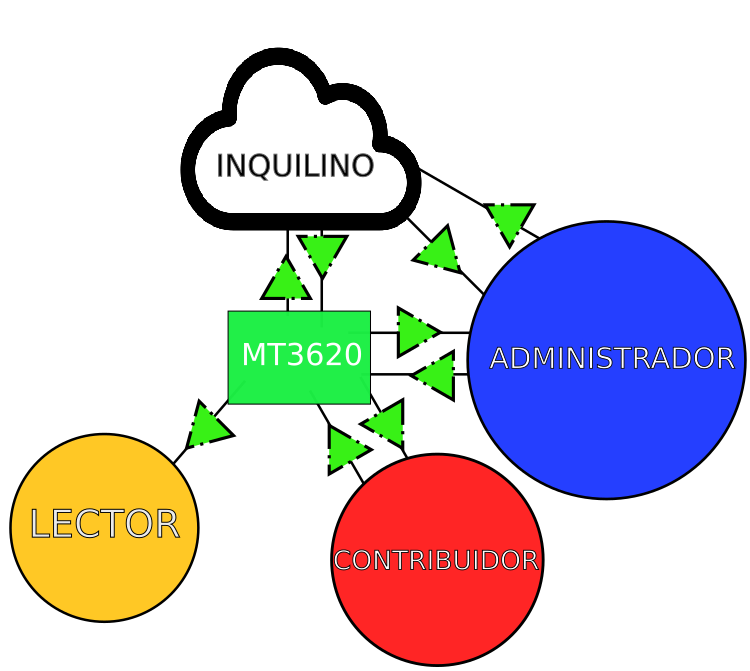
\includegraphics[scale = 1.25]{tenant}
	\caption{Organización de desarrollo}
\end{figure}

Primero, en la terminal de tu sistema operativo, deberás de registrar un correo (que use los servicios de Microsoft) a la plataforma: 
\begin{verbatim}
	azshpere register-user --new-user <correo-electronico>
\end{verbatim}

Inicia sesión con el siguiente comando:
\begin{verbatim}
	azsphere login
\end{verbatim}

\subsubsection{Registro del dispositivo}
\textit{Tener en cuenta que esta operación NO se pude revertir.}
\linebreak
\linebreak
Primero necesitas tener el dispositivo conectado a tu ordenador. Después se necesita ver si tu cuenta no tiene algún inquilino disponible; esto se hace con el comando:
\begin{verbatim}
	azsphere tenant list
\end{verbatim}
Si aparecen uno o varios inquilinos, solo sería seleccionar uno con el comando:
\begin{verbatim}
	azsphere tenant select --tenant <nombre o ID del tenant>
\end{verbatim}

En el caso de que no salga ninguno, tienes dos opciones: pides al administrador de un inquilino que agregue tu cuenta y te dé un rol con los siguientes comandos:
\begin{verbatim}
azsphere register-user --new-user <correo-electronico>
azsphere role add --role <rol> --user <correo-electronico>
\end{verbatim}
O se crea un inquilino:
\begin{verbatim}
	azsphere tenant create --name <nombre-del-tenant>
\end{verbatim}
Al crear un nuevo inquilino, tu usuario tendrá el rol de administrador por defecto.


\subsubsection{Roles en un inquilino}
\begin{itemize}
	\item 
	Administrador: tiene acceso completo a todos los dispositivos y operaciones, también puede añadir o eliminar a otros usuarios. Se recomienda solo dos cuentas con este rol.
	\item 
	Contribuidor: Pueden registrar dispositivos, hacer cambios o implementaciones, pero no eliminar operaciones. Básicamente, pueden hacer desarrollo en el kit, pero no administrar el inquilino.
	\item 
	Lector: Tiene la capacidad de leer la información del inquilino, los dispositivos registrados, implementaciones y errores. Este rol es apropiado para el mantenimiento.
	
\end{itemize}

\subsection{Conectando el MT3620 a Internet}
Se tiene que conectar el microcontrolador a una red de internet para que pueda recibir actualizaciones y pueda comunicarse al centro de IoT de Azure. Esto se hace a partir de la IDE que estés usando.
Si quieres comprobar primero que tu microcontrolador este conectado a internet utiliza:

\begin{verbatim}
	azsphere device wifi show-status
\end{verbatim}

\subsubsection{Visual Studio}
\begin{itemize}
	\item
	Conectas la Azure Sphere a tu computadora.
	\item 
	En el menú selecciona Ver $\rightarrow$ Otra Ventana $\rightarrow$ Explorador de Azure Sphere.
	(View $\rightarrow$ Other Windows $\rightarrow$ Azure Sphere Explorer)
	
	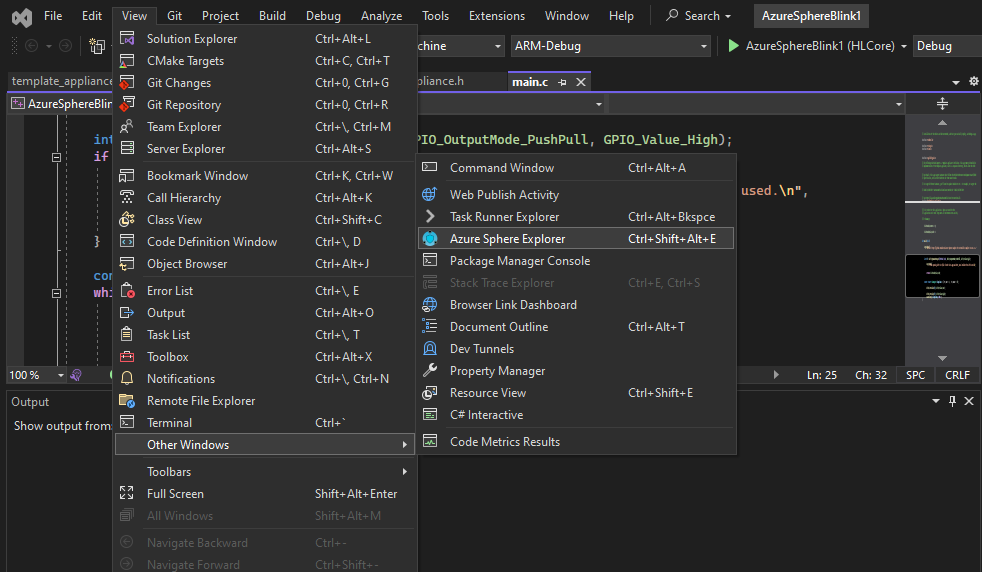
\includegraphics[width=\textwidth,height=\textheight,keepaspectratio]{VS2}
	\pagebreak
	\item 
	Desglosa el dispositivo del menú. 
	
	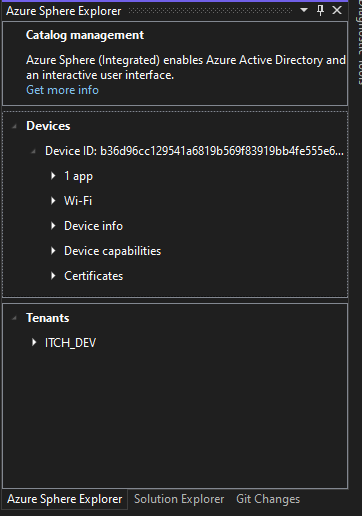
\includegraphics[width=\textwidth,height=\textheight,keepaspectratio]{VS3}
	\pagebreak
	\item 
	Expande la sección de Wi-fi.

	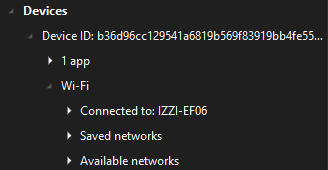
\includegraphics[width=\textwidth,height=\textheight,keepaspectratio]{VS4}
	\item 
	Si en uno de los elementos te indica como desconectado, entonces expande la sección de redes disponibles.
	\item 
	Selecciona la red que deseas e ingresa la contraseña.
\end{itemize}
\pagebreak
\subsubsection{Visual Studio Code}
\begin{itemize}
	\item
	Conectas la Azure Sphere a tu computadora.
	\item 
	Presiona el botón de Ver $\rightarrow$ Abrir Vista... . (View $\rightarrow$ Open View...)
	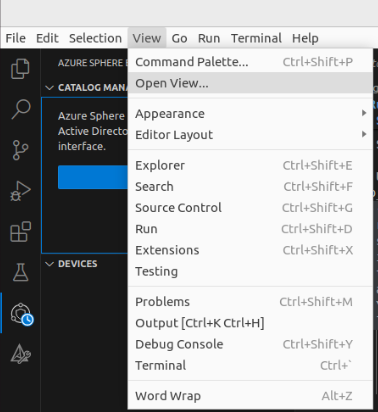
\includegraphics[width=\textwidth,height=\textheight,keepaspectratio]{VSCode2}
	\item 
	Escriba la palabra Azure y seleccione Azure Sphere Explorer; aparecerá un menú en la sección lateral del VSCode.  
	\linebreak
	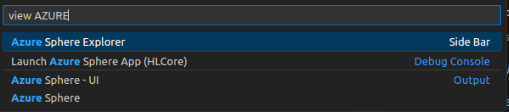
\includegraphics[width=\textwidth,height=\textheight,keepaspectratio]{VSCode2-5}
	\pagebreak
	\item 
	Desglosa el dispositivo del menú. 

	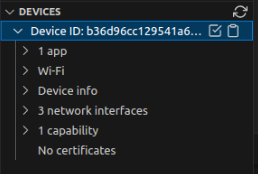
\includegraphics[width=\textwidth,height=\textheight,keepaspectratio]{VSCode3}
	\item 
	Expande la sección de Wi-fi.

	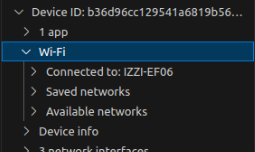
\includegraphics[width=\textwidth,height=\textheight,keepaspectratio]{VSCode4}
	\item 
	Si en uno de los elementos te indica como desconectado, entonces expande la sección de redes disponibles.
	\item 
	Selecciona la red que deseas e ingresa la contraseña.
\end{itemize}

\subsection{Habilitar desarrollo del microcontrolador}
Por último tienes que habilitar el modo desarrollador para poder grabar algo en el MCU. Esto se hace desde la terminal con el siguiente comando:
\begin{verbatim}
azsphere device enable-development
\end{verbatim}

\subsection{Compilar y cargar un programa al MC}
	\section{Desarrollo en la MT3620}
Esta tablilla tiene dos tipos de aplicaciones que se le pueden desarrollar: la de alto nivel y la de tiempo real. A pesar de que sean dos tipos de implementación, estas se pueden desarrollar con total comodidad en la IDE que hayas elegido.


\subsection{Alto nivel}
Este tipo de aplicación es requerida en cada dispositivo Azure Sphere. El código corre en el sistema operativo de Azure Sphere. Puedes usar librerías de aplicaciones.

Estas pueden:
\begin{itemize}
	\item
	Configurar los periféricos de la Azure Sphere como el GPIO, UARTs y otras interfaces.
	\item 
	Comunicarse con las aplicaciones de tiempo real.
	\item 
	Comunicarse por medio del Internet.
\end{itemize}

Este es el uso normal del microcontrolador. Este tipo solo puede acceder a librerías que permita Microsoft, no tiene permitido el acceso mediante shell o archivos del I/O.

\subsection{Tiempo Real}
En este tipo de aplicación está más cerca del metal, por lo que en este puedes interactuar y configurar con los puertos del microcontrolador. También puedes implementar un sistema operativo en tiempo real y estas aplicaciones pueden comunicarse con las de alto nivel.

\section{Definiciones de hardware}
Desarrollar en este tipo de tarjetas de desarrollo tiene sus beneficios, uno de estos son las definiciones de hardware, estas definen la locación de los periféricos. Ayudan a una mejor compresión en el código, en estas tarjetas hay dos archivos para modificar esto, primero están los especificados por el fabricante, estos ya vienen en el SDK de la Azure Sphere en el directorio \textit{ProgramFiles(x86)\textbackslash Microsoft Azure Sphere SDK\textbackslash HardwareDefinitions} en Windows y \textit{/opt/azurespheresdk/HardwareDefinitions} en Linux. También existen las definiciones de aplicaciones especificas, estas se crean a partir de las especificadas por el fabricante y asignan identificadores que se usan de referencia, así el cambio de una tablilla a otra es más sencillo.
Estos archivos están escritos en json, y su formato es el siguiente.
\begin{lstlisting}[language = json, firstnumber=1]
{
	"Metadata": //Informacion sobre el archivo
	{
		"Type": "Azure Sphere Hardware Definition",
		"Version": 1
	},
	"Description": //Informacion sobre la tablilla o modulo
	{
		"Name": "<nombre de la tablilla o modulo>",
		"MainCoreHeaderFileTopContent": [
		"/* Copyright (c) <vendor name> Todos los derechos reservados.",
		" <Informacion de alguna licencia> */",
		"",
		"// This header contains the peripheral pinout definitions for
		the",
		"// <name of board or module>"
		]
	},
	"Imports" : [ {"Path": ""} //Direccion del archivo de definicion de hardware para definir sobre ella
	],
	"Peripherals": [ //Los perifericos que se van usar para la aplicacion
	{"Name": "<Nombre en el codigo>", "Type": "<Tipo de periferico>", "Mapping": "<El nombre del periferico en el archivo importado>", "Comment": "<Informacion a destacar>"},
	]
}
\end{lstlisting}

\subsection{Creando el encabezado}
Después de tener definidas los componentes a utilizar, se puede generar el archivo .h, en la terminal se pone el siguiente comando:
\begin{verbatim}
azsphere hardware-definition generate-header --hardware-definition-file
<filename> 
\end{verbatim}
\begin{figure}[h]
	\centering
	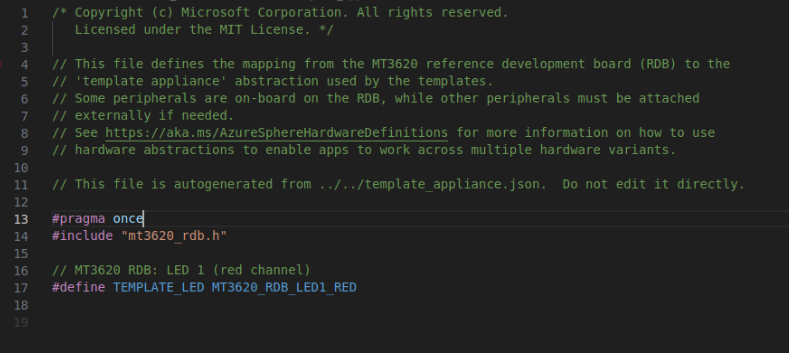
\includegraphics[width=\textwidth,height=\textheight,keepaspectratio]{header}
	\caption{Ejemplo de archivo header del proyecto blink}
\end{figure}

\textbf{Nota}: por defecto, el archivo encabezado creará una carpeta que siempre será el subdirectorio de la locación donde se encuentre el archivo JSON.
\subsection{Declaración de aplicación}
También conocido como las capacidades de aplicación, es un archivo que indica los recursos a utilizar de la aplicación, cada proyecto debe de tener uno. En esta deben estar todos los puertos y módulos que se van a utilizar de la tarjeta, los recursos se declaran basados en la definición de hardware que se explicó anteriormente. Esta declaración siempre se encuentra en el archivo app\_manifest.json
\begin{figure}[h]
	\centering
	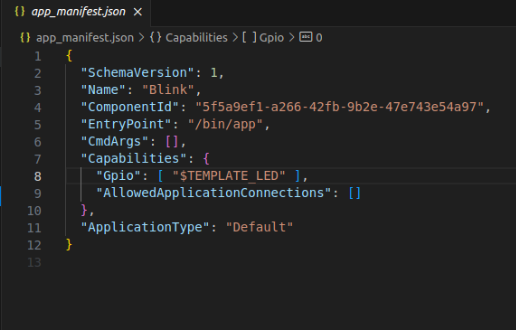
\includegraphics[scale=.60]{appmanifest}
	\caption{Ejemplo app\_manifest.json del proyecto blink}
\end{figure}
\subsection{Usando las definiciones del SDK}

\begin{enumerate}
	\item Se tiene que generar un proyecto en blanco, después en el archivo CMakeList.txt se anade la siguiente linea:
	\begin{verbatim}
	azsphere_target_hardware_definition(${PROJECT_NAME} 
	TARGET_DEFINITION "mt3620_rdb.json") 
	\end{verbatim}
	\item 
	En el archivo main.c incluir el archivo tipo cabecera correspondiente.
	\begin{lstlisting}[language = C, firstnumber=0]
#include  "hw/mt3620_rdb.h"
	\end{lstlisting}
	\item 
	Cambiar el application manifest anadiendo el periferico ha utilizar, por ejemplo para usar un GPIO, se pone lo siguiente
	\begin{lstlisting}[language = json, firstnumber=0]
"Capabilities": 
{  
	"Gpio": [ "$MT3620_RDB_LED1_RED" ] 
}
	\end{lstlisting}
	\item 
	Compilar el proyecto
\end{enumerate}


	\section{Perifericos}
En esta seccion se mostrara algunas especificaciones del periferico y el como anadirlos en los archivos de cabecera y configuraciones en el app manifest.\par
Al desarrollar aplicaciones en RT, se utiliza uno de los ARM Cortex M4 que tiene el integrado. Ya existen unos \href{https://github.com/CodethinkLabs/mt3620-m4-drivers/tree/master}{drivers} para la MT3620, o puedes usar los registros de memoria que están documentados (\href{https://d86o2zu8ugzlg.cloudfront.net/mediatek-craft/documents/mt3620/MT3620-Datasheet-v1.7.pdf}{datasheet} y
\href{https://d86o2zu8ugzlg.cloudfront.net/mediatek-craft/documents/MT3620-M4-User-Manual.pdf}{manual}) por el fabricante. A la hora de elegir un periférico en el app manifest, es casi lo mismo. Ahora, para seleccionar un puerto, se elige el identificador ``maping'' del archivo mt3620.json (véase capítulo 6).


\subsection{GPIO}
\subsubsection{HL}
\begin{lstlisting}[language = C, firstnumber=0]
	#include <applibs/gpio.h>
\end{lstlisting}
\begin{lstlisting}[language = json, firstnumber=0]	
	"Capabilities": 
	{  
		"Gpio": [ "$MACRO_DEL_GPIO" ] 
	}
\end{lstlisting}
\subsubsection{RT}
\begin{lstlisting}[language = json, firstnumber=0]	
	"Capabilities": {
		"Gpio": [ 8, 12 ]
	}
\end{lstlisting}

\subsection{ADC}
Ocho canales de 12 bits, usando un voltaje de referencia a 2.5 V internos o 1.8 V externos.
\subsubsection{HL}
\begin{lstlisting}[language = C, firstnumber=0]
	#include <applibs/adc.h>
\end{lstlisting}
\begin{lstlisting}[language = json, firstnumber=0]	
	"Capabilities": 
	{  
		"Adc": [ "$MACRO_DEL_ADC" ] 
	}
\end{lstlisting}
\subsubsection{RT}
\begin{lstlisting}[language = json, firstnumber=0]	
	"Capabilities": {
		"Adc": [ "ADC-CONTROLLER-0" ]  }
\end{lstlisting}

\subsection{UART}
\subsubsection{HL}
\begin{lstlisting}[language = C, firstnumber=0]
	#include "applibs_versions.h"
	#include <applibs/uart.h>
\end{lstlisting}
\begin{lstlisting}[language = json, firstnumber=0]	
	"Capabilities": 
	{  
		"Uart": [ "$MACRO_DEL_UART" ] 
	}
\end{lstlisting}
\subsubsection{RT}
\begin{lstlisting}[language = json, firstnumber=0]	
	"Capabilities": {
		"Uart": [ "ISU0" ]
	}
\end{lstlisting}

\subsection{PWM}
\subsubsection{HL}
\begin{lstlisting}[language = C, firstnumber=0]
	#include <applibs/pwm.h>
\end{lstlisting}
\begin{lstlisting}[language = json, firstnumber=0]	
	"Capabilities": 
	{  
		"Pwm": [ "$MACRO_DEL_PWM" ] 
	}
\end{lstlisting}
\subsubsection{RT}
\begin{lstlisting}[language = json, firstnumber=0]	
	"Capabilities": 
	{  
		"Pwm": [ "PWM-CONTROLLER-0" ] 
	}
\end{lstlisting}

\subsection{SPI}
\subsubsection{HL}
\begin{lstlisting}[language = C, firstnumber=0]
	#include "applibs_versions.h"
	#include <applibs/spi.h>
\end{lstlisting}
\begin{lstlisting}[language = json, firstnumber=0]	
	"Capabilities": {  
		"SpiMaster": [ "$MACRO_DEL_SPI_ISU0", $MACRO_DEL_SPI_ISU1" ]
	}
\end{lstlisting}
\subsubsection{RT}
\begin{lstlisting}[language = json, firstnumber=0]	
	"Capabilities": {
		"SpiMaster": [ "ISU0", "ISU1" ] }
\end{lstlisting}

\subsection{I2C}
\subsubsection{HL}
\begin{lstlisting}[language = C, firstnumber=0]
	#include "applibs_versions.h"
	#include <applibs/i2c.h>
\end{lstlisting}
\begin{lstlisting}[language = json, firstnumber=0]		"Capabilities":
	{  
		"I2C": [ "$MACRO_DEL_I2C" ] 
	}
\end{lstlisting}
\subsubsection{RT}
\begin{lstlisting}[language = json, firstnumber=0]	
	"Capabilities": {
		"I2C": [ "ISU0" ]
	}
\end{lstlisting}

	\section{IoT}
En esta seccion se demostrara como usar el Azure Sphere para conectarse al servicio Azure IoT Hub de Microsoft.
\subsection{Registro en Azure}
Registre una cuenta gratuita en \href{https://azure.microsoft.com/es-mx/free}{Azure}. Para esto,	 necesita obligatoriamente un numero telefónico y una tarjeta de crédito o débito para verificar su identidad.

Ahora se tiene que crear un IoT Hub, este es un servicio de la nube que funciona como un centro de comunicación entre distintos aplicaciones IoT. Para crearlo, en el panel de Azure, selecciona Create a resource.
\begin{figure}[h]
	\centering
	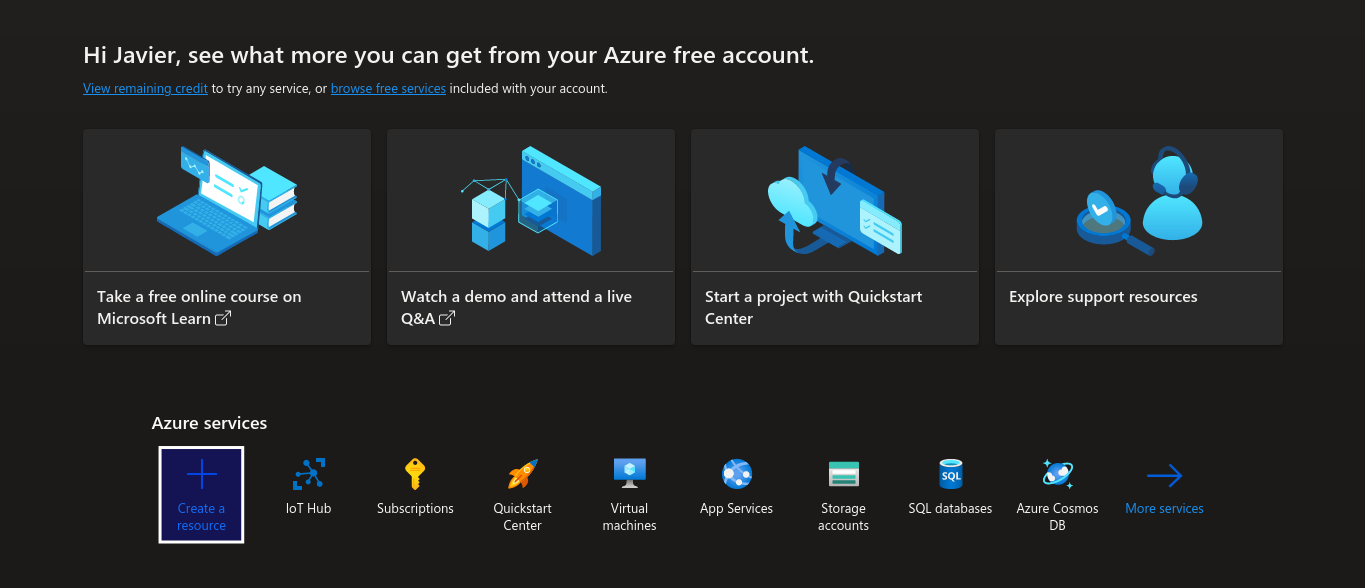
\includegraphics[width=0.75\textwidth,height=\textheight,keepaspectratio]{Azure1}
\end{figure}
En la pagina de Create a resource, en la sección de categorías, elige Internet of Things y presiona IoT Hub.
\begin{figure}[h]
	\centering
	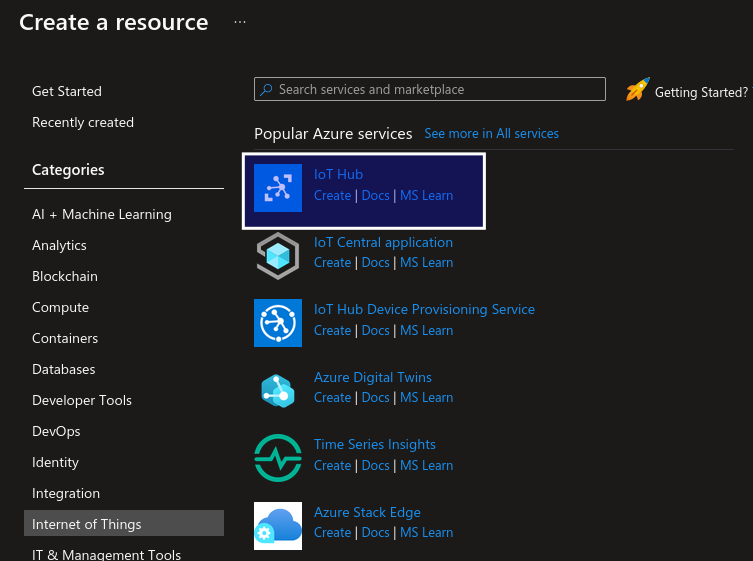
\includegraphics[width=0.75\textwidth,height=\textheight,keepaspectratio]{Azure2}
\end{figure}
Llena todos los datos para el registro de tu IoT Hub. El resource group lo puedes crear ahi mismo. La región elige la de tu preferencia. El nivel elige gratuito. El nombre del Hub solo tienen que ser letras. Al tener todo listo da click en review + create y para confirmar create.
\begin{figure}[h]
	\centering
	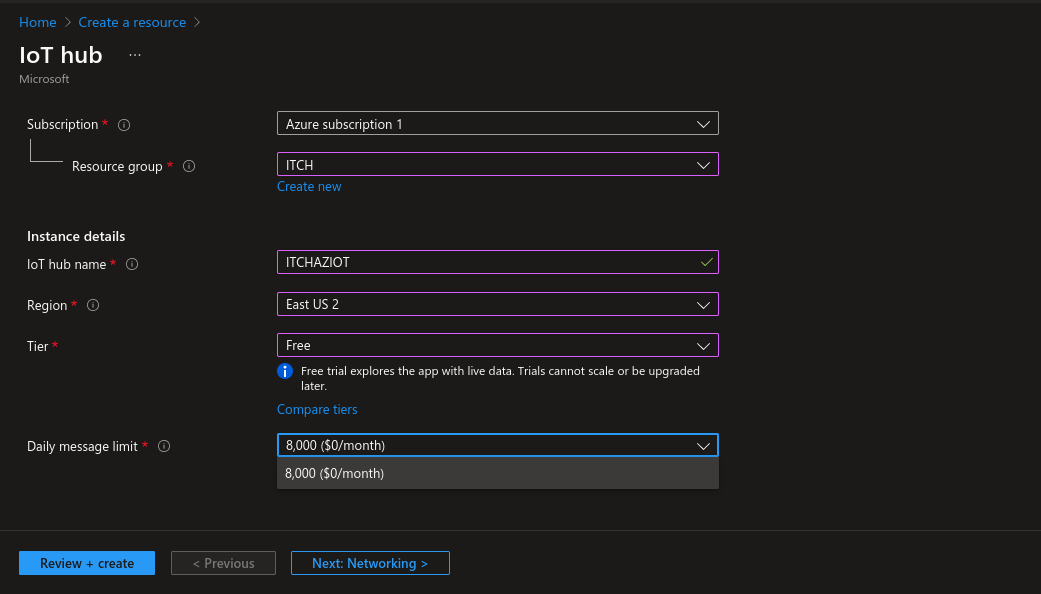
\includegraphics[width=0.75\textwidth,height=\textheight,keepaspectratio]{Azure3}
\end{figure}
\subsection{Certificado del Azure Sphere}
En la terminal, ejecutar el siguiente comando.
\begin{verbatim}
	azsphere ca-certificate download --destination CAcertificate.cer
\end{verbatim}
Esto generara un certificado en el directorio que se encuentre la terminal.
\subsection{Subir el certificado al Iot hub}
Navega al IoT hub que creaste.

\begin{figure}[h]
	\centering
	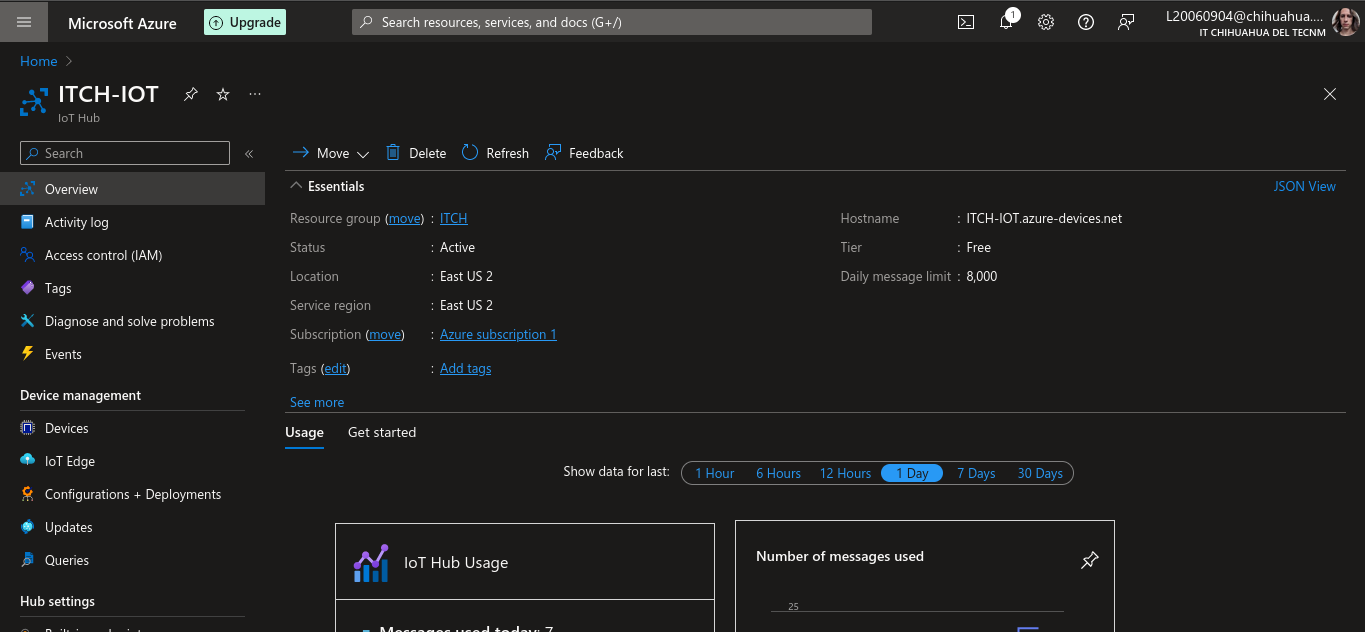
\includegraphics[width=0.75\textwidth,height=\textheight,keepaspectratio]{Azure4}
\end{figure}
\pagebreak
Ve a la sección de certificados.
\begin{figure}[h]
	\centering
	
\includegraphics[width=0.75\textwidth,height=0.35\textheight,keepaspectratio]{Azure5}
\end{figure}

Ya estando en la sección, presiona el botón de add.
\begin{figure}[h]
	\centering
	
\includegraphics[width=0.9\textwidth,height=\textheight,keepaspectratio]{Azure6}
\end{figure}
\pagebreak

Agrega el nombre, el archivo del certificado y marca la casilla de "Set certificate status to verified on upload".
\begin{figure}[h]
	\centering
	
\includegraphics[width=0.9\textwidth,height=\textheight,keepaspectratio]{Azure7}
\end{figure}
\subsection{Agregar dispositivo}
En la pagina del IoT Hub, navega a la sección de dispositivos.
\begin{figure}[h]
	\centering
	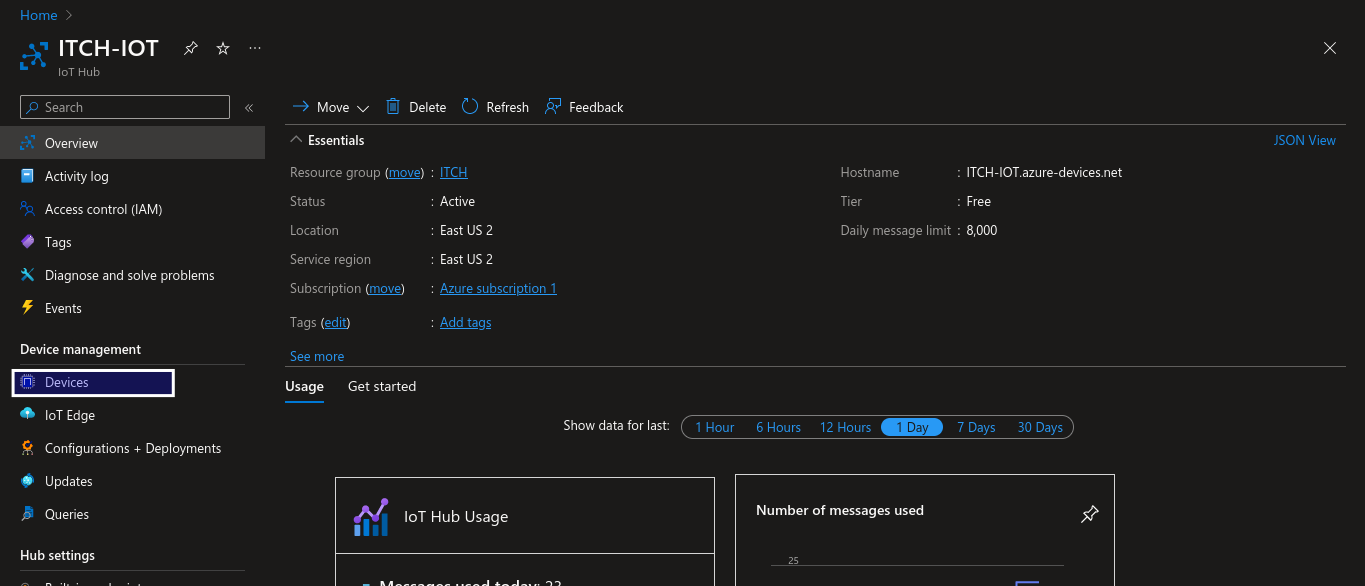
\includegraphics[width=0.75\textwidth,height=\textheight,keepaspectratio]{Azure8}
\end{figure}

Estando en la sección, presiona el botón de add device
\begin{figure}[h]
	\centering
	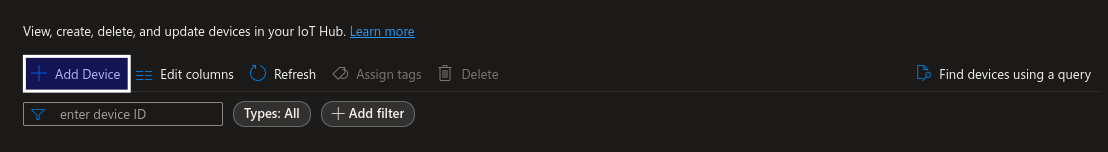
\includegraphics[width=0.9\textwidth,height=\textheight,keepaspectratio]{Azure9}
\end{figure}
\pagebreak

Agrega el id del dispositivo, este lo obtienes en la terminal con el siguiente comando (El dispositivo debe estar conectado a la computadora):
\begin{verbatim}
	azsphere device show-attached
\end{verbatim}
En el tipo de autenticación eliges X.509 CA Signed. Despues presiona save.
\begin{figure}[h]
	\centering
	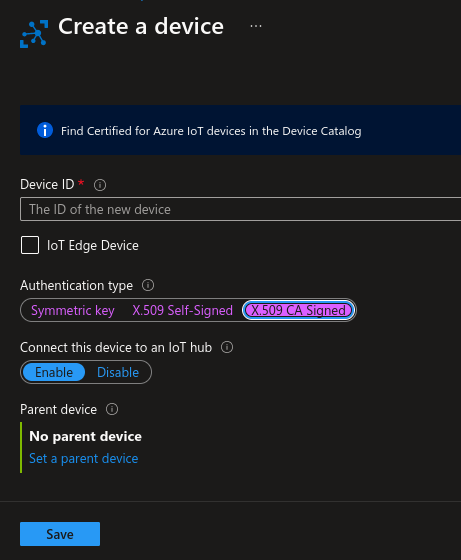
\includegraphics[width=0.9\textwidth,height=\textheight,keepaspectratio]{Azure10}
\end{figure}

	\section{Ejemplos}
\subsection{Diagrama de conexiones}
Para el correcto funcionamiento de estos ejemplos, primero se tiene que hacer las siguientes conexiones:
\begin{figure}[h]
	\centering
	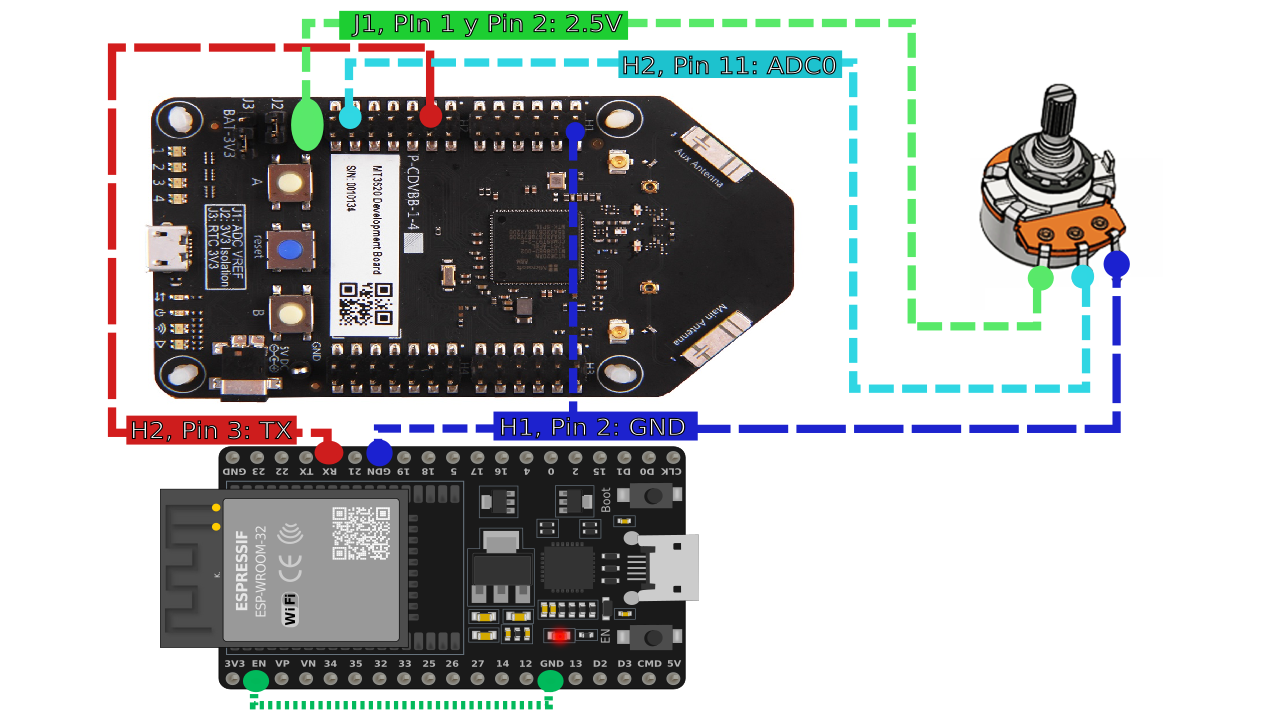
\includegraphics[scale=.40]{DiagramaDeConexion}
	\caption{Diagrama de conexiones.}
\end{figure}
\linebreak
El potenciómetro hará que varié la lectura del ADC. El ESP32 se está usando como un UART a USB, lo necesitas conectar a una computadora y leerlo en una terminal serial. Este nos dará los mensajes que envié el MT3620. El ESP32 se puede reemplazar por adaptadores UART a USB si se desea.
\pagebreak
\subsection{Códigos}
\begin{itemize}
	\item 
	\href{https://github.com/Javier20060904/ejemplo_HL}{ejemplo\textunderscore HL}: Este programa consiste en el uso de ADC, GPIO y UART usando las API's de Azure Sphere en alto nivel.
	\item
	\href{URL}{ejemplo\textunderscore RT}
\end{itemize}



	\section{Recursos para profundizar}
\begin{itemize}
	\item
	\href{https://github.com/Azure/azure-sphere-samples}{Azure Sphere Samples}
	\item 
	\href{https://github.com/Azure/azure-sphere-tools}{Azure Sphere Tools}
	\item 
	\href{https://github.com/Azure/azure-sphere-samples}{Azure Sphere Samples}
	\item 
	\href{https://github.com/Azure/azure-sphere-gallery}{Azure Sphere Gallery}
	\item 
	\href{https://github.com/MicrosoftDocs/Azure-Sphere-Developer-Learning-Path}{Azure Sphere Developer Learning Path}
	\item 
	\href{https://github.com/Azure-Samples/Azure-RTOS-on-Azure-Sphere-Mediatek-MT3620}{Azure RTOS on Azure Sphere}
	\item 
	\href{https://github.com/CodethinkLabs/mt3620-m4-samples/}{MT3620 M4 Samples}
	\item 
	\href{https://github.com/CodethinkLabs/mt3620-m4-drivers}{MT3620 M4 Drivers}
	\item 
	\href{https://github.com/MediaTek-Labs/mt3620_m4_software/}{MT3620 M4 Driver and Real-Time Application Sample Code}
	\item 
	\href{https://github.com/avnet-iotconnect/iotc-sphereos-sdk}{IoTConnect C SDK for Azure Sphere}
	\item 
	\href{https://github.com/xiongyu0523/azure-sphere-aws-iot-device-sdk-embedded-c}{Azure Sphere AWS IoT SDK}
\end{itemize}
	\section{Referencias}
[1] Prabhushyja, “Azure sphere documentation,” Microsoft Learn, \href{https://learn.microsoft.com/en-us/azure-sphere/}{https://learn.microsoft.com/en-us/azure-sphere/} (accessed Sep. 29, 2023). \par
[2] “Azure Sphere MT3620 Development Kit | Seeed Studio Wiki,” wiki.seeedstudio.com, Jan. 12, 2023. \href{https://wiki.seeedstudio.com/Azure_Sphere_MT3620_Development_Kit/}{https://wiki.seeedstudio.com/Azure\_Sphere\_MT3620\_Develop-
ment\_Kit/}
(accessed Sep. 29, 2023). \par
[3] MEDIATEK, \href{bhttps://d86o2zu8ugzlg.cloudfront.net/mediatek-craft/documents/mt3620/MT3620-Datasheet-v1.7.pdf}{“MT3620 DATASHEET.”}  MEDIATEK, Jan. 26, 2021 
‌	
\end{document}
